\documentclass{refart}
\usepackage[utf8]{inputenc}
\usepackage[english]{babel}
\usepackage{graphicx}
\usepackage{url}

\title{Guide to Vaspirin 1.1}
\author{Instituto Tecnológico de Aeronáutica\\
	Group of Semiconductor Materials and Nanotechnology\\
	Daniel S. Koda\thanks{\texttt{danielskoda@gmail.com}}\\
	Ivan Guilhon\thanks{\texttt{ivanguilhonn@gmail.com}}}
\date{May 2016}

\begin{document}

\maketitle

\begin{abstract}
	Vaspirin is a post-processsing tool for VASP made in Python. Its goals are to simplify the analysis of simulations, make standard and beautiful figures easily and create a continuous development and centralization of the tool throughout the years for the Group of Semiconductor Materials and Nanotechnology (GMSN). This document describes the capabilities of the software and provides a beginner's guide to its utilization. We cover the installation of the script and demonstrate the use of this tool with examples, such as band structure and density of states plotting.
\end{abstract}

\tableofcontents

\section{Introduction}

\subsection{About Vaspirin}

\marginlabel{Origins:} Vaspirin has been created to unify and document scripts made by members of GMSN in a way which benefits both experienced students with its pragmatic and well-tested approach as well as beginner undergraduate students by lessening the initial difficulties of juggling programming languages, solid state physics, undergraduate studies \textsc{and} simulations at once.

\marginlabel{Authors:} Daniel S. Koda (MSc student in 2016) and Ivan Guilhon (PhD student in 2016) are responsible for the beginning of this project and the documentation.

	\marginlabel{Software:} The raw code and the installation package can be found at: \url{https://github.com/gmsn-ita/vaspirin.git}. New versions will be constantly updated in this link.

\subsection{Installation}

\marginlabel{Requirements:} Vaspirin uses Python 3 as standard language. The packages \texttt{numpy}, \texttt{matplotlib}, \texttt{scipy}, \texttt{pylab}, and \texttt{setuptools} are required in order to take full advantage of Vaspirin. XMGrace is also recommended to plot \texttt{.bfile} scripts generated by Vaspirin. \texttt{git} is necessary if you want to contribute to the software. Please use your package manager to install these packages before proceeding with the installation.

\marginlabel{Installing:} Directly download the Vaspirin code from \url{https://github.com/gmsn-ita/vaspirin.git} or simply execute:\\
 \texttt{git clone https://github.com/gmsn-ita/vaspirin.git}.
 
Once downloaded, go to the directory \texttt{vaspirin/} and execute execute:\\
\texttt{\# python setup.py install} or \texttt{\$ sudo python setup.py install}

If Python 3 is not the default Python language in your operating system (confirm by executing \texttt{python --version}), you may want to try:\\
\texttt{\# python3 setup.py install}

From this point on, you can execute \texttt{vaspirin} as a normal command-line interface software.

\section{Running Vaspirin}

\subsection{Flags}

\marginlabel{Introduction:} Vaspirin was created with an eye to flexibility. Therefore, most of its features are activated by running  the script with flags starting with a dash \texttt{-}. All possibilities are briefly listed here and demonstrated in the examples section. Further development may take advantage of these functions and classes put together in order to make a more complex script.

\marginlabel{\texttt{-bs outcarFile}} Reads the eigenvalues from the \texttt{outcarFile} specified. If the file is not given, the default \texttt{OUTCAR} file is read from the current directory.

\marginlabel{\texttt{-dos doscarFile}} Reads the density of states from the \texttt{doscarFile} specified. If the file is not given, the default \texttt{DOSCAR} file is read from the current directory.

\marginlabel{\texttt{-char procarFile}} Reads the character of simulated band structures from the \texttt{procarFile} specified. If the file is not given, the default \texttt{PROCAR} file is read from the current directory.

\marginlabel{\texttt{-proj procarFile PROJECTION}} Reads the character of simulated band structures from the \texttt{procarFile} specified and the projection description in the \texttt{PROJECTION} file. If the file is not given, the default \texttt{PROCAR, PROJECTION} file are read from the current directory. The format of the \texttt{PROJECTION} file are specified in subsection \ref{sec:projection}.

\marginlabel{\texttt{-compare OUTCAR1 OUTCAR2 }} Plot two different OUTCARs in a same band structure. Assumes both calculations are made with the same k-points line, imported from the KPOINTS file.

\marginlabel{\texttt{-plot}} Plots the specified function using XMGrace. A \texttt{.dat} (or a directory replete with \texttt{.dat} files) and a \texttt{.bfile} are generated. The \texttt{.bfile} should be executed as batch by XMGrace after using Vaspirin so that the plot can be fully generated.

\marginlabel{\texttt{-pyplot}} Plots the specified function using PyPlot.

\marginlabel{\texttt{-quiet}} Do not print the introduction message.

\marginlabel{\texttt{-yaxis y1 y2}} Define the y-scaling as the range [$\min(\texttt{y1},\texttt{y2})$, $\max$(\texttt{y1},\texttt{y2})].

\marginlabel{\texttt{-ignore N}} Ignore the first N k-points when plotting band structures. Useful for HSE calculations, in which k-points for band structures are included in the same file as the self-consistent k-points mesh.

\marginlabel{\texttt{-ref reference}} Define an arbitrary reference for the 0 eV level in band structures. Recognized arguments are: \texttt{vbm}, \texttt{efermi}, \texttt{e-fermi} and any floating-point number. Default: \texttt{vbm}.

\marginlabel{\texttt{-soc}} Import OUTCAR with spin-orbit coupling for setting correctly the valence band based on occupations.

\marginlabel{\texttt{-interpolate N }} Linearly interpolate N points between each point in band structures. Useful for coloring projected band structures. Default: 0

\marginlabel{\texttt{-markersize size}} Changes the marker size for projected and character band structures. Default: 0.5.

\marginlabel{\texttt{-ps psFile}} Enables direct exporting from XMGrace to PS files. Requires the use of a XMGrace command after \texttt{vaspirin}



\subsection{Standards requiring manual entry}\label{sec:projection}

\marginlabel{\texttt{KPOINTS} header:} To create a band structure specifying symmetry k-points, a header describing which are these special k-points should be written in the \texttt{KPOINTS} file. The header has the following format:\\
\texttt{SymPoint1 Index1, SymPoint2 Index2, SymPoint3 Index3, \ldots}

A specific example is shown in section \ref{sec:example-bands}.

\marginlabel{\texttt{PROJECTION} file:} Projected band structures are creating by summing all contributions from atoms which belong to specified materials. Therefore, which atoms are part of each material is an information supplied by the user. The \texttt{PROJECTION} file is responsible for conveying that data to \texttt{vaspirin}. It is a plain text file with the following format:

\texttt{Material1Label atomsBelongingToMaterial1\\Material2Label atomsBelongingToMaterial2\\ \vdots}

An example of application of this technique is shown in section \ref{sec:example-proj}.

\marginlabel{\texttt{.dat} files:} These files are output from \texttt{vaspirin} and contain information about the simulation loaded. For band structures (\texttt{eigenv.dat}), this file is a double-column table, in which the first column is the normalized k-point (based on the length and the size of the Brillouin zone) and the second is the corresponding eigenvalue. Bands are organized in blocks. In cases such as projection and orbital character, a folder named \texttt{bands\_character} or \texttt{bands\_projected} is created, and one \texttt{.dat} file is written for each band. This allows plotting special band structures with XMGrace.

\marginlabel{\texttt{.bfile} files:} This kind of file contain batch instructions for plotting data with XMGrace. They should be executed with this software, for example:\\
\texttt{xmgrace -batch bands.bfile}

\section{Tutorial}

In this section, actual examples of calculations will be supplied in order to clarify the use of \texttt{vaspirin}. The files for this example are available in the folder \texttt{tests/} in the \texttt{vaspirin} directory. No VASP simulations will be done at this point.

\subsection{Plotting standard band structures}\label{sec:example-bands}

\marginlabel{Changing the directory:} As a first step, the default configurations from \texttt{vaspirin} are used. This is the more favorable situation, in which \texttt{vaspirin} is executed in the same folder as the VASP simulation. Therefore, all files have their default name and are all in the same directory. To start using \texttt{vaspirin}, please change your directory to that of interest.

\marginlabel{\texttt{KPOINTS} header:} The \texttt{KPOINTS} file must specify the path made in the band structure calculation, as well as their indexes. In this case, 130 k-points were used to form the entire path, distributed so that the $\Gamma$ point were the 1st and the 130th points, the M point was the 41th point and the K point was the 70th point. Thus, the \texttt{KPOINTS} header should be:\\
\texttt{G 0, M 40, K 69, G 129}

\marginlabel{Executing \texttt{vaspirin} and obtaining the data:} To plot a simple band structure using \texttt{vaspirin}, just execute:\\
\texttt{vaspirin -bs -plot}

This tells \texttt{vaspirin} to acquire band structure data (\texttt{-bs} flag) from the default \texttt{OUTCAR} file and then plot the correspondent bands. This generate the files \texttt{eigenv.dat} and \texttt{bands.bfile}.

\marginlabel{Generating the bands using XMGrace:} Finally, you can create the plot by executing:\\
\texttt{xmgrace -batch bands.bfile}

The result of these operations for the given example files is shown in Fig. \ref{fig:bs-plot}.

\begin{figure}[h!]
	\centering
	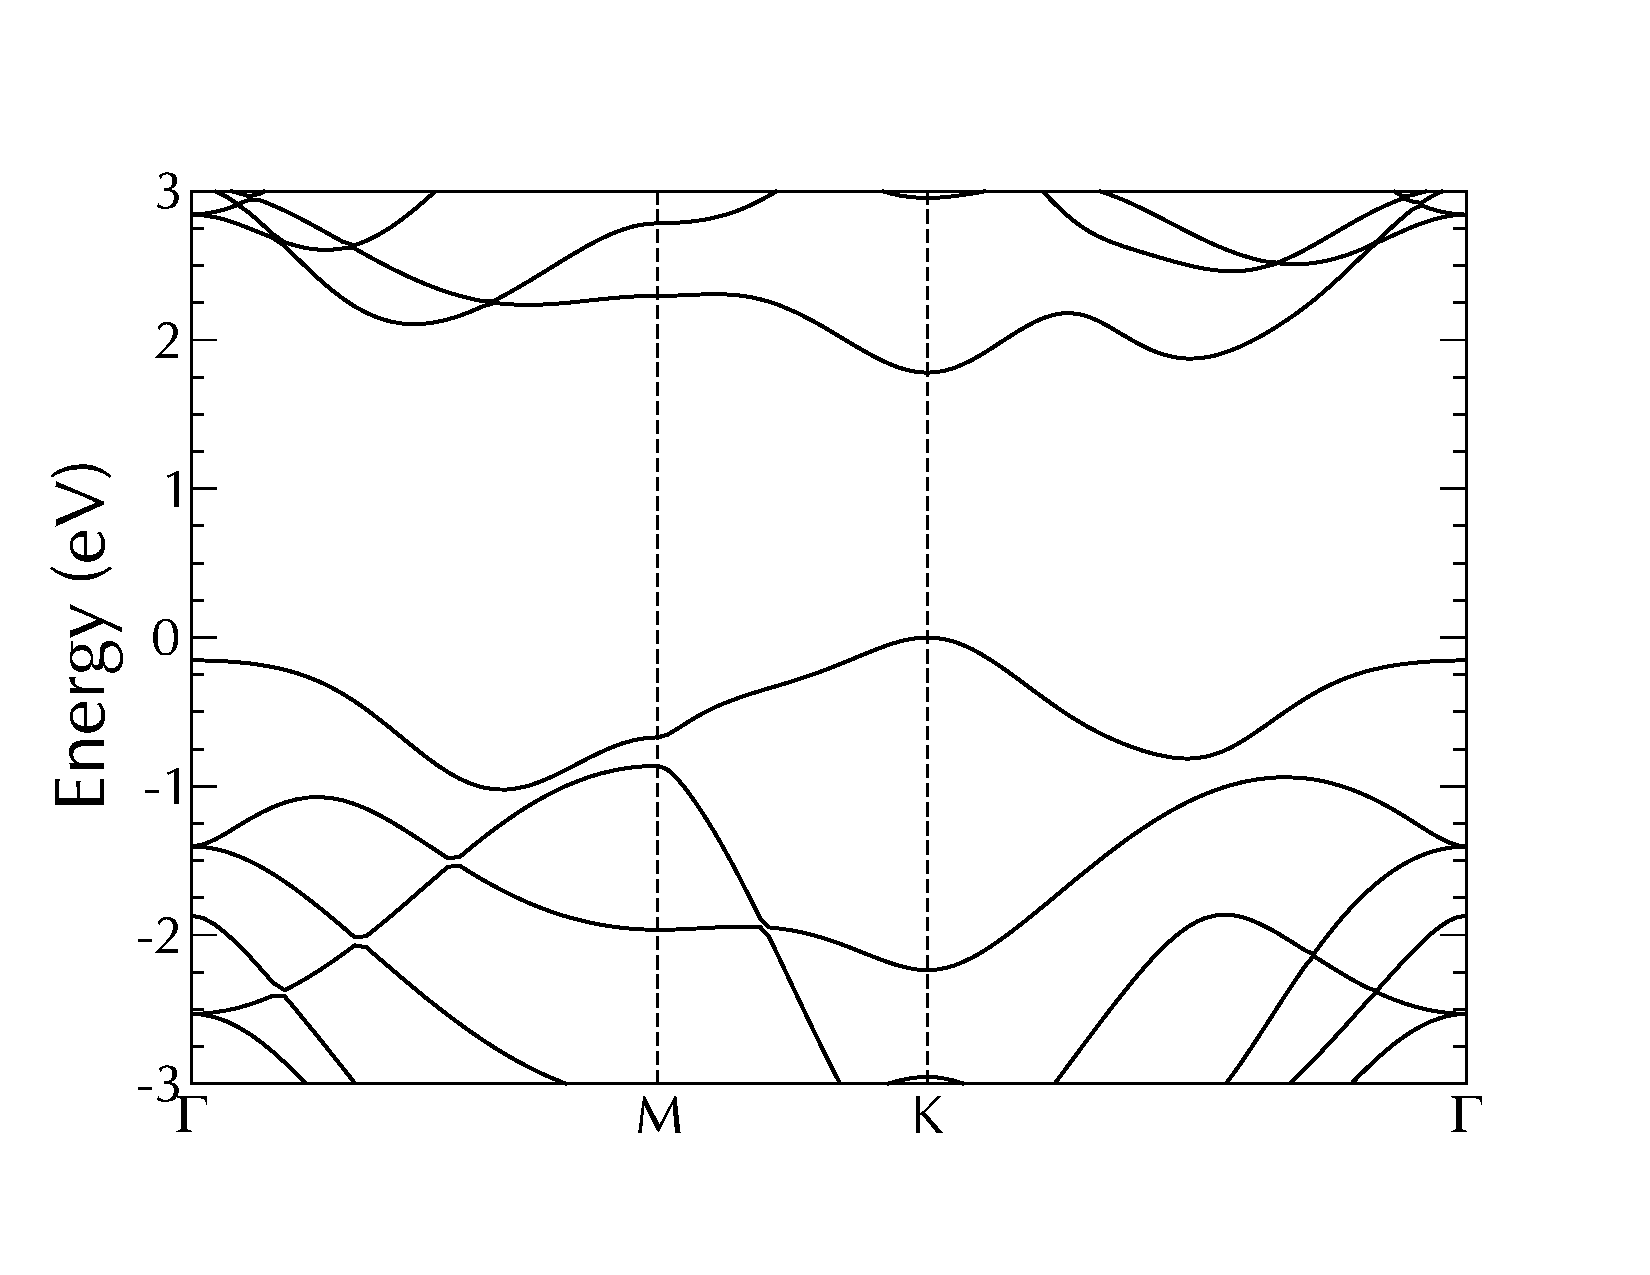
\includegraphics[width=\textwidth]{img/bs-plot.pdf}
	\caption{Example of a monolayer MoS$_2$ band structure plotted using \texttt{vaspirin -bs -plot}.}
	\label{fig:bs-plot}
\end{figure}

\marginlabel{Changing the y-axis scale:} \texttt{vaspirin} puts the 0 eV reference on the top of the valence band (additional features for Fermi energy, vacuum level and custom energies are being implemented). If the default range of [-3,3] eV is not enough, it is possible to customize these values simply by using the tag \texttt{-yaxis}. Continuing the example above with this tag:\\
\texttt{vaspirin -bs -plot -yaxis -2 4}

This new band structure is shown in Fig. \ref{fig:bs-plot-yaxis}.

\begin{figure}[h!]
	\centering
	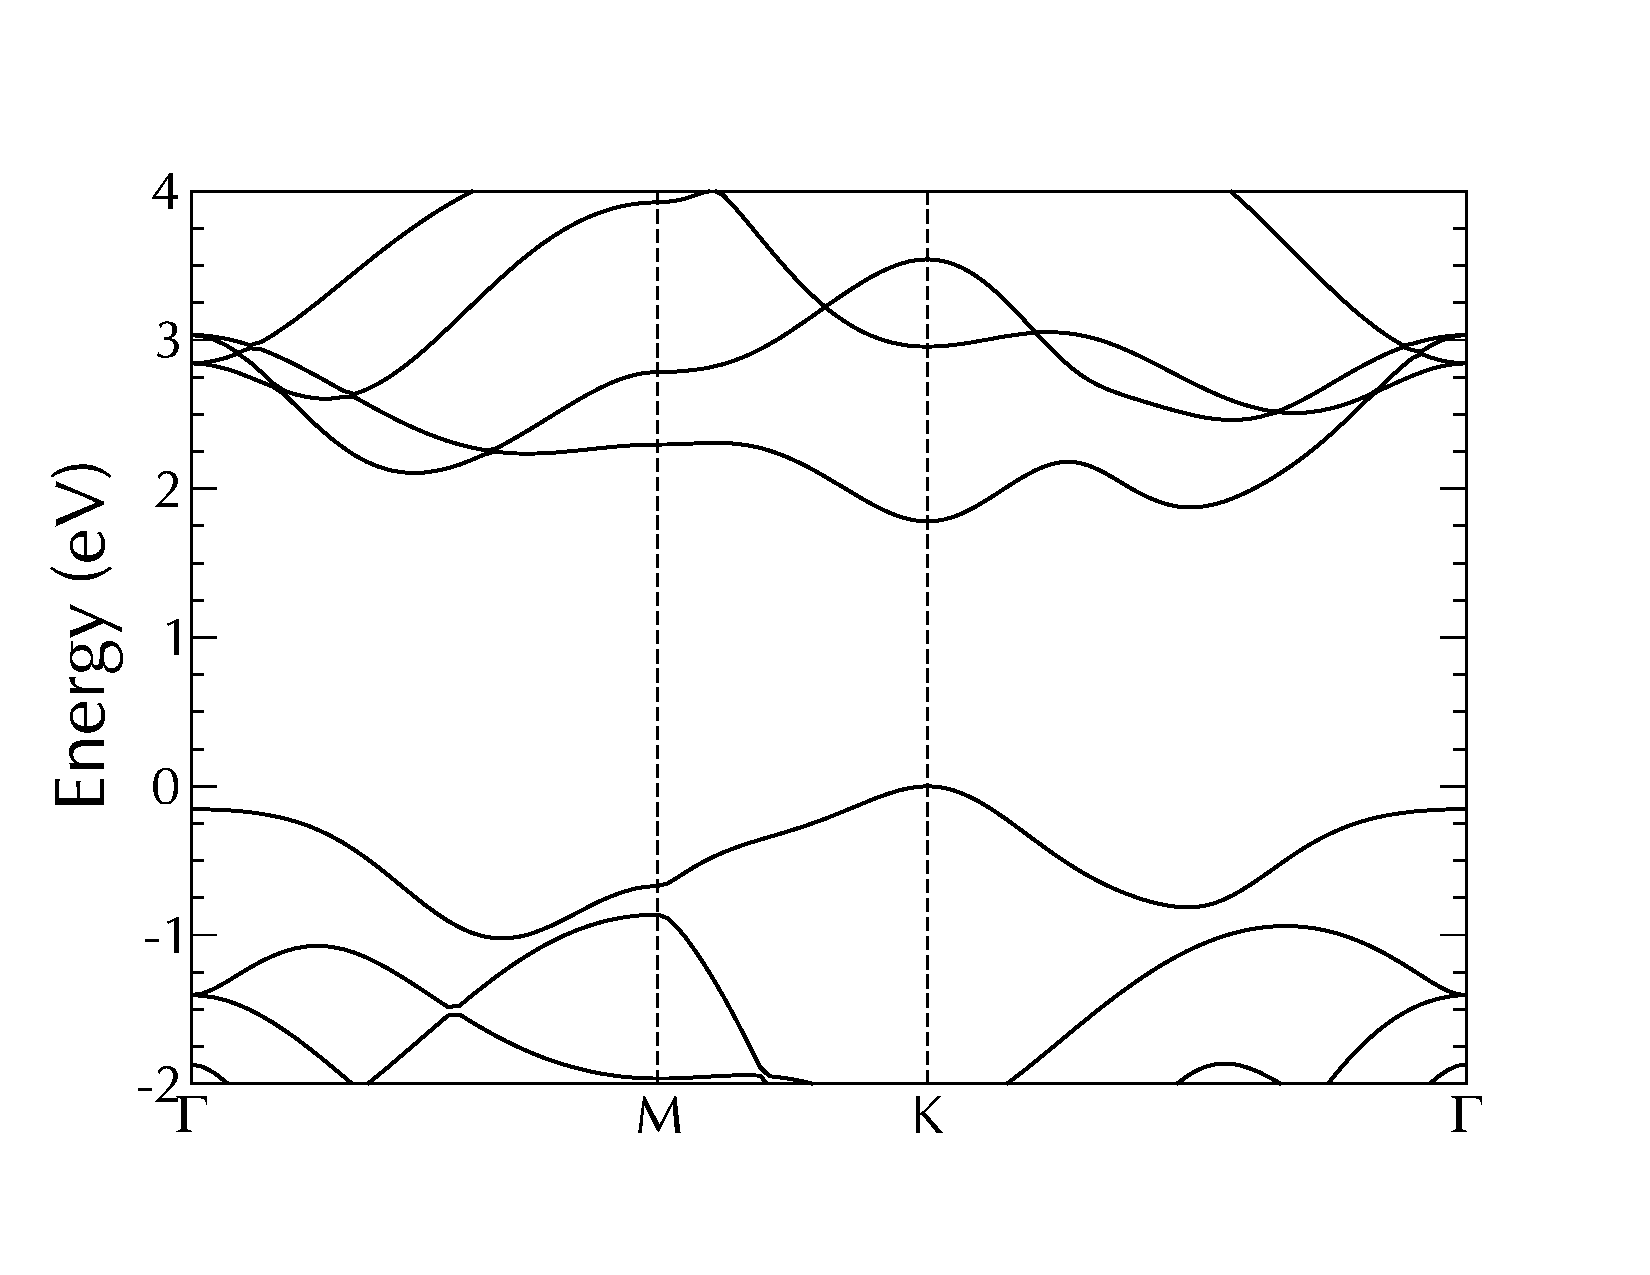
\includegraphics[width=\textwidth]{img/bs-plot-yaxis.pdf}
	\caption{Example of a monolayer MoS$_2$ band structure plotted using \texttt{vaspirin -bs -plot -yaxis -2 4}.}
	\label{fig:bs-plot-yaxis}
\end{figure}

It should be noted that \texttt{vaspirin} does not care about the order in which the numbers after \texttt{-yaxis} are written. Therefore, running \texttt{vaspirin -bs -plot -yaxis 4 -2} would yield exactly the same result.

\marginlabel{Running files other than the default:} If your files have names other than the default for VASP, or if they are in other directory, it suffices to call \texttt{vaspirin} with arguments specified after the tags, as in:\\
\texttt{vaspirin -bs mos2/OUTCAR -plot}

\subsection{Plotting band structures projected on orbitals}

In many cases, it is useful to analyze the system based on the formation of the bands via orbitals. \texttt{vaspirin} allows this kind of analysis to be done. Creating this requires a \texttt{PROCAR} file, which has the contributions of all points from the band structure.

\marginlabel{Generating band structures with orbital character:} To create band structures with orbital character, \texttt{vaspirin} should be executed with the \texttt{-char} tag active:\\
\texttt{vaspirin -bs -char -plot}

This loads the default \texttt{OUTCAR} and \texttt{PROCAR} files from the current directory. To use another files as input, an argument can be specified after the flags \texttt{-bs} and \texttt{-char}. \texttt{vaspirin} outputs the data to the folder \texttt{bands\_character/} and the XMGrace batch \texttt{bandsCharacter.bfile}.

\marginlabel{Plotting with XMGrace:} To plot the resulting file with XMGrace, execute the following line:\\
\texttt{xmgrace -batch bandsCharacter.bfile}

The result is shown in Fig. \ref{fig:bs-char}.

\begin{figure}[h!]
	\centering
	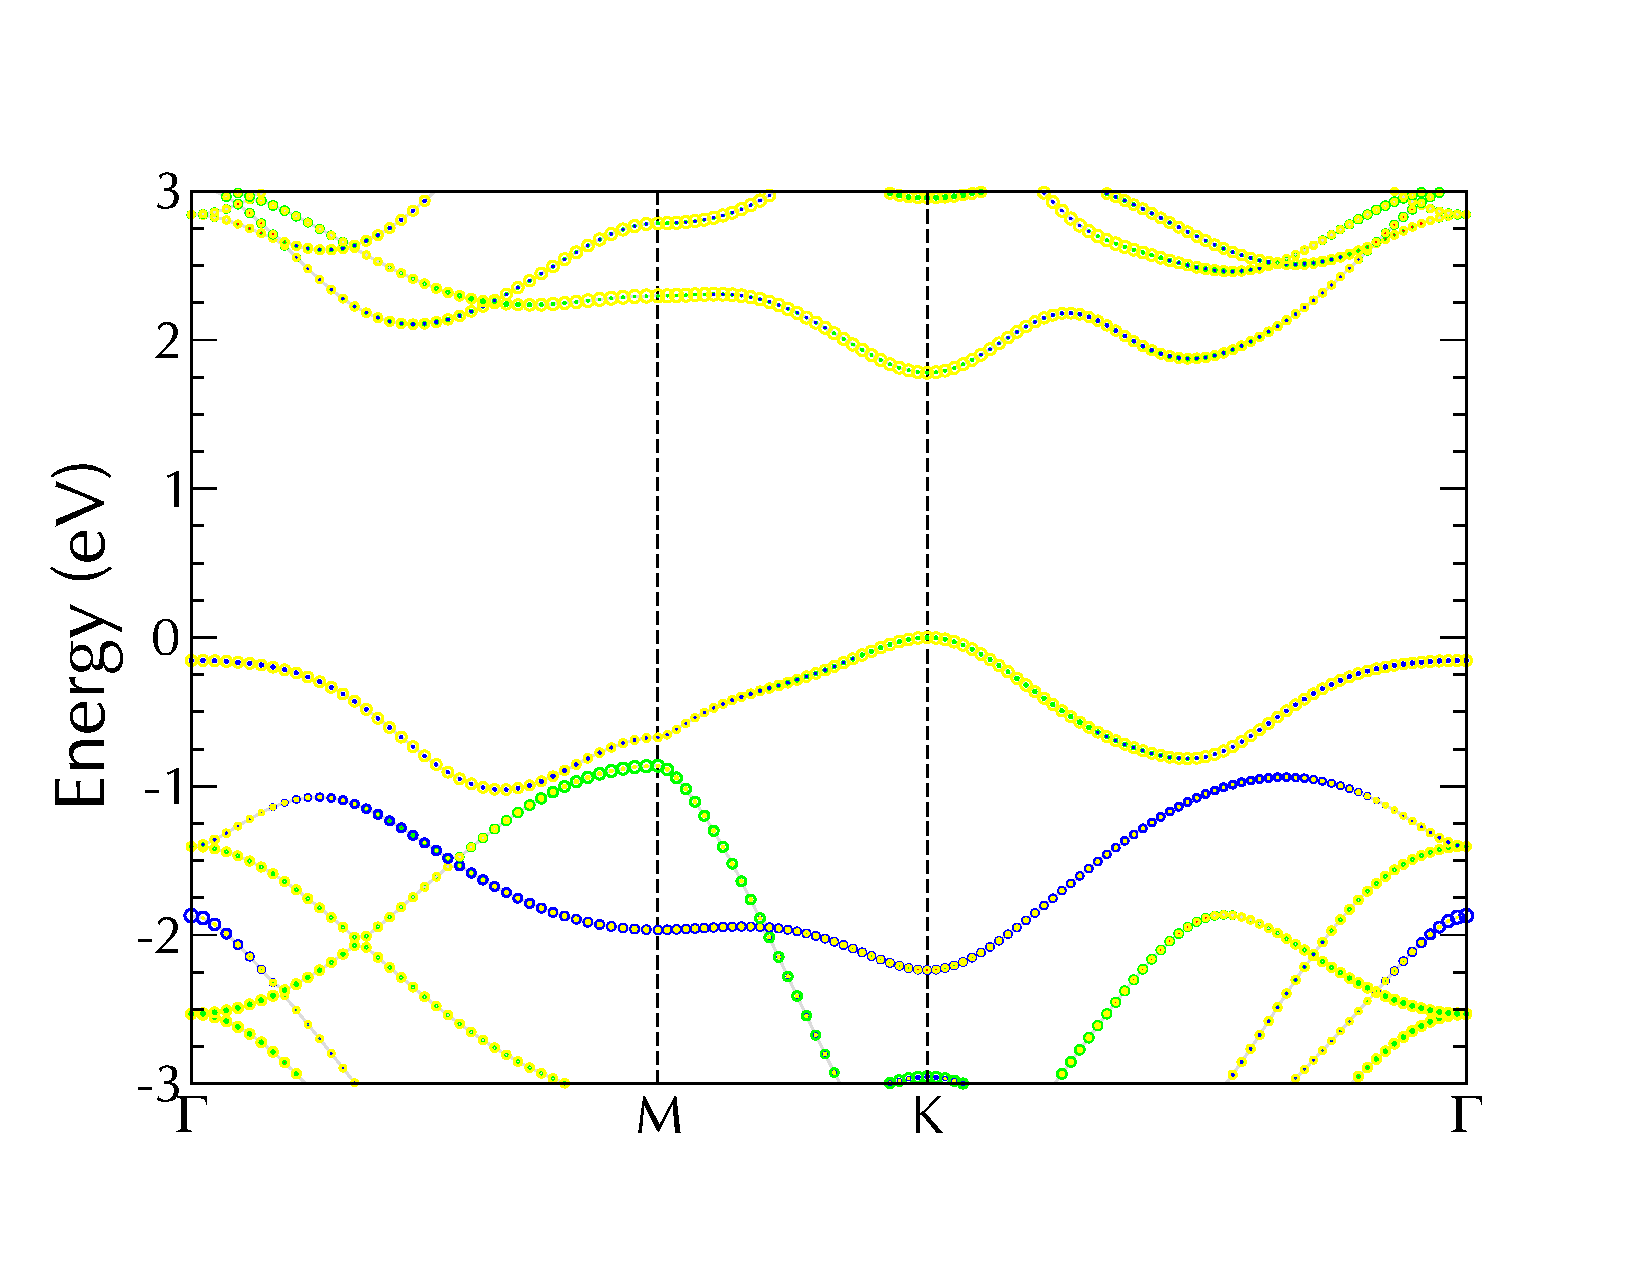
\includegraphics[width=\textwidth]{img/bs-char.pdf}
	\caption{Example of a monolayer MoS$_2$ band structure plotted using \texttt{vaspirin -bs -char -plot}. Red, green, blue and yellow circles depict contributions from $s$, $p_x + p_y$, $p_z$ and $d$ orbitals, respectively.}
	\label{fig:bs-char}
\end{figure}

\marginlabel{Interpreting the figure:} Orbital contributions scale the colored circular markers in the band structure. Therefore, bigger circles imply predominance of the specific orbital to the formation of the band exactly in that k-point. Red, green, blue and yellow circles depict contributions from $s$, $p_x + p_y$, $p_z$ and $d$ orbitals, respectively.

\subsection{Plotting band structures projected on specific ions} \label{sec:example-proj}

Sometimes, as in van der Waals heterostructures, it is useful to know which bands come from each of its constituents. This not only helps visualize effects on electronic structures but also creates a pleasant interpretation to the viewer.

\marginlabel{Creating the \texttt{PROJECTION} file:} The \texttt{PROJECTION} file is a user-made text file which specifies which atoms compose each material. In the case of the MoS$_2$, only two different atoms are simulated, and they are part of a single material. If we wanted to analyze contributions of the molybdenum atom to the bands formation, as well as the sulfur atom to it, we would have to build the following \texttt{PROJECTION} file:

\texttt{Mo 1\\S 2..3}

A $2 \times 2$ supercell of MoS$_2$, therefore with 12 atoms inside it, would have the following \texttt{PROJECTION} file:

\texttt{Mo 1..4\\S 5..12}

Another equivalent way of specifying the information above would be:

\texttt{molybdenum 1,2,3,4\\sulfur 5,6,7..12}

Atoms must be numbered according to their order in the \texttt{POSCAR} file and be separated by commas. The \texttt{7..12} entry indicates all atoms between the 7th and the 12th (including these both) belong to the material named \texttt{sulfur}. The labels can be chosen arbitrarily and is more like a guide for humans than a useful information for \texttt{vaspirin}. All atoms should be specified in the \texttt{PROJECTION} file.

\marginlabel{Generating the data with \texttt{vaspirin}:} To use the simulation and the specification from the \texttt{PROJECTION} file, just run the following command:\\
\texttt{vaspirin -bs -proj -plot}

A folder named \texttt{bands\_projected} and a XMGrace batch named \texttt{bandsProjected.bfile} are created upon the execution of this command.

\marginlabel{Plotting with XMGrace:} To plot the resulting file with XMGrace, execute the following line:\\
\texttt{xmgrace -batch bandsProjected.bfile}

The result is shown in Fig. \ref{fig:bs-proj}.

\begin{figure}[h!]
	\centering
	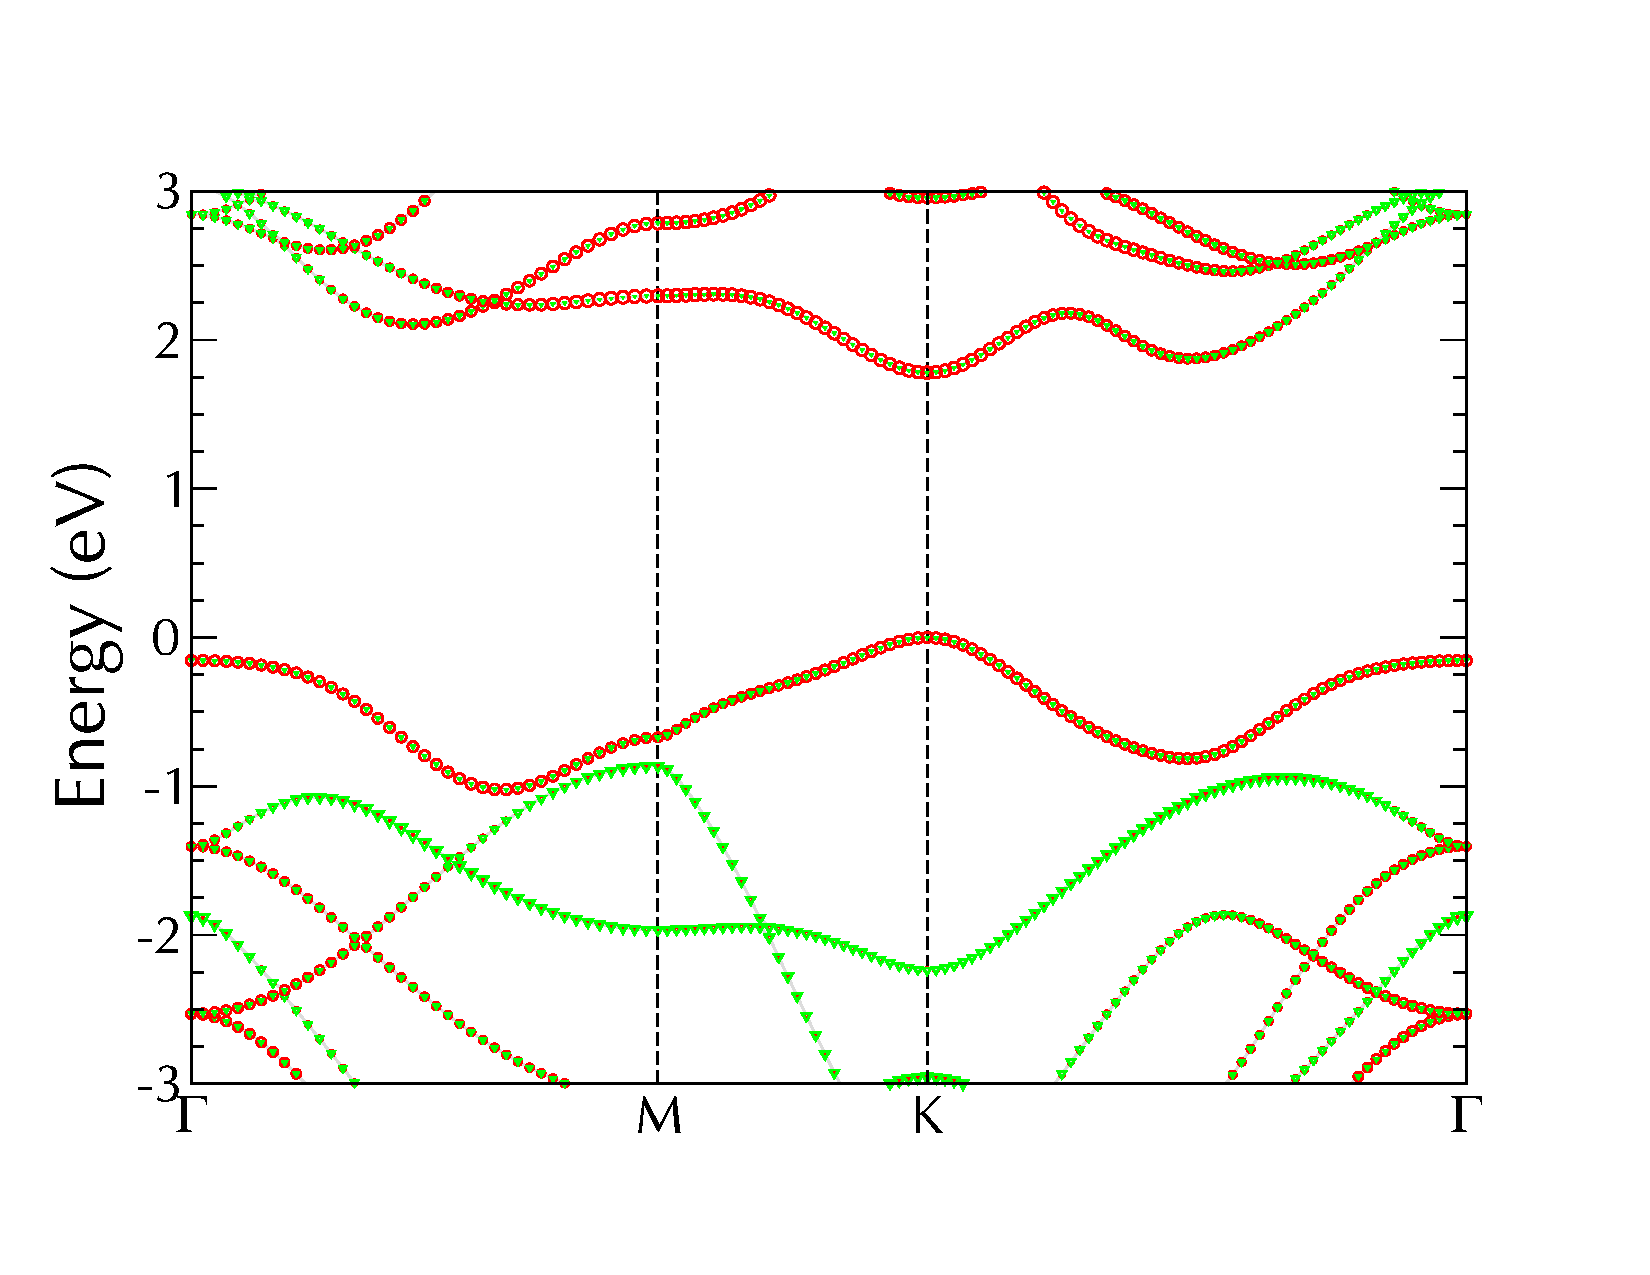
\includegraphics[width=\textwidth]{img/bs-proj.pdf}
	\caption{Example of a monolayer MoS$_2$ band structure plotted using \texttt{vaspirin -bs -proj -plot}. Red and green markers depict contributions from Mo and S atoms, respectively.}
	\label{fig:bs-proj}
\end{figure}

\marginlabel{Interpreting the figure:} Each material contributions scale the colored markers in the band structure. Therefore, bigger markers imply predominance of the specific material to the formation of the band exactly in that k-point. The materials are represented with red, green, blue, yellow, brown, gray, violet, cyan, etc. according to their order in the \texttt{PROJECTION} file.

\subsection{Comparing two different band structures}

Comparing two different band structures using \texttt{vaspirin} is an easy task. \texttt{vaspirin} still has a limitation and assumes that only bands executed with the same k-points mesh will be compared. Otherwise, results cannot have any meaning.

\marginlabel{Comparing band structures:} To compare band structures, \texttt{vaspirin} should be executed with the \texttt{-compare} tag instead of the \texttt{-bs} tag:\\
\texttt{vaspirin -compare -plot}

This loads the default \texttt{OUTCAR1} and \texttt{OUTCAR2} files from the current directory. To use another files as input, an argument can be specified after the flags \texttt{-compare}, as in \texttt{vaspirin -compare mat1-OUTCAR mat2-OUTCAR}. \texttt{vaspirin} outputs the data to two \texttt{.dat} files, nominally \texttt{eigenv1.dat} and \texttt{eigenv2.dat}, and the XMGrace batch to \texttt{bandsComparison.bfile}.

\marginlabel{Plotting with XMGrace:} To plot the resulting file with XMGrace, execute the following line:\\
\texttt{xmgrace -batch bandsComparison.bfile}

An example is shown in Fig. \ref{fig:compare-bs}.

\begin{figure}[h!]
	\centering
	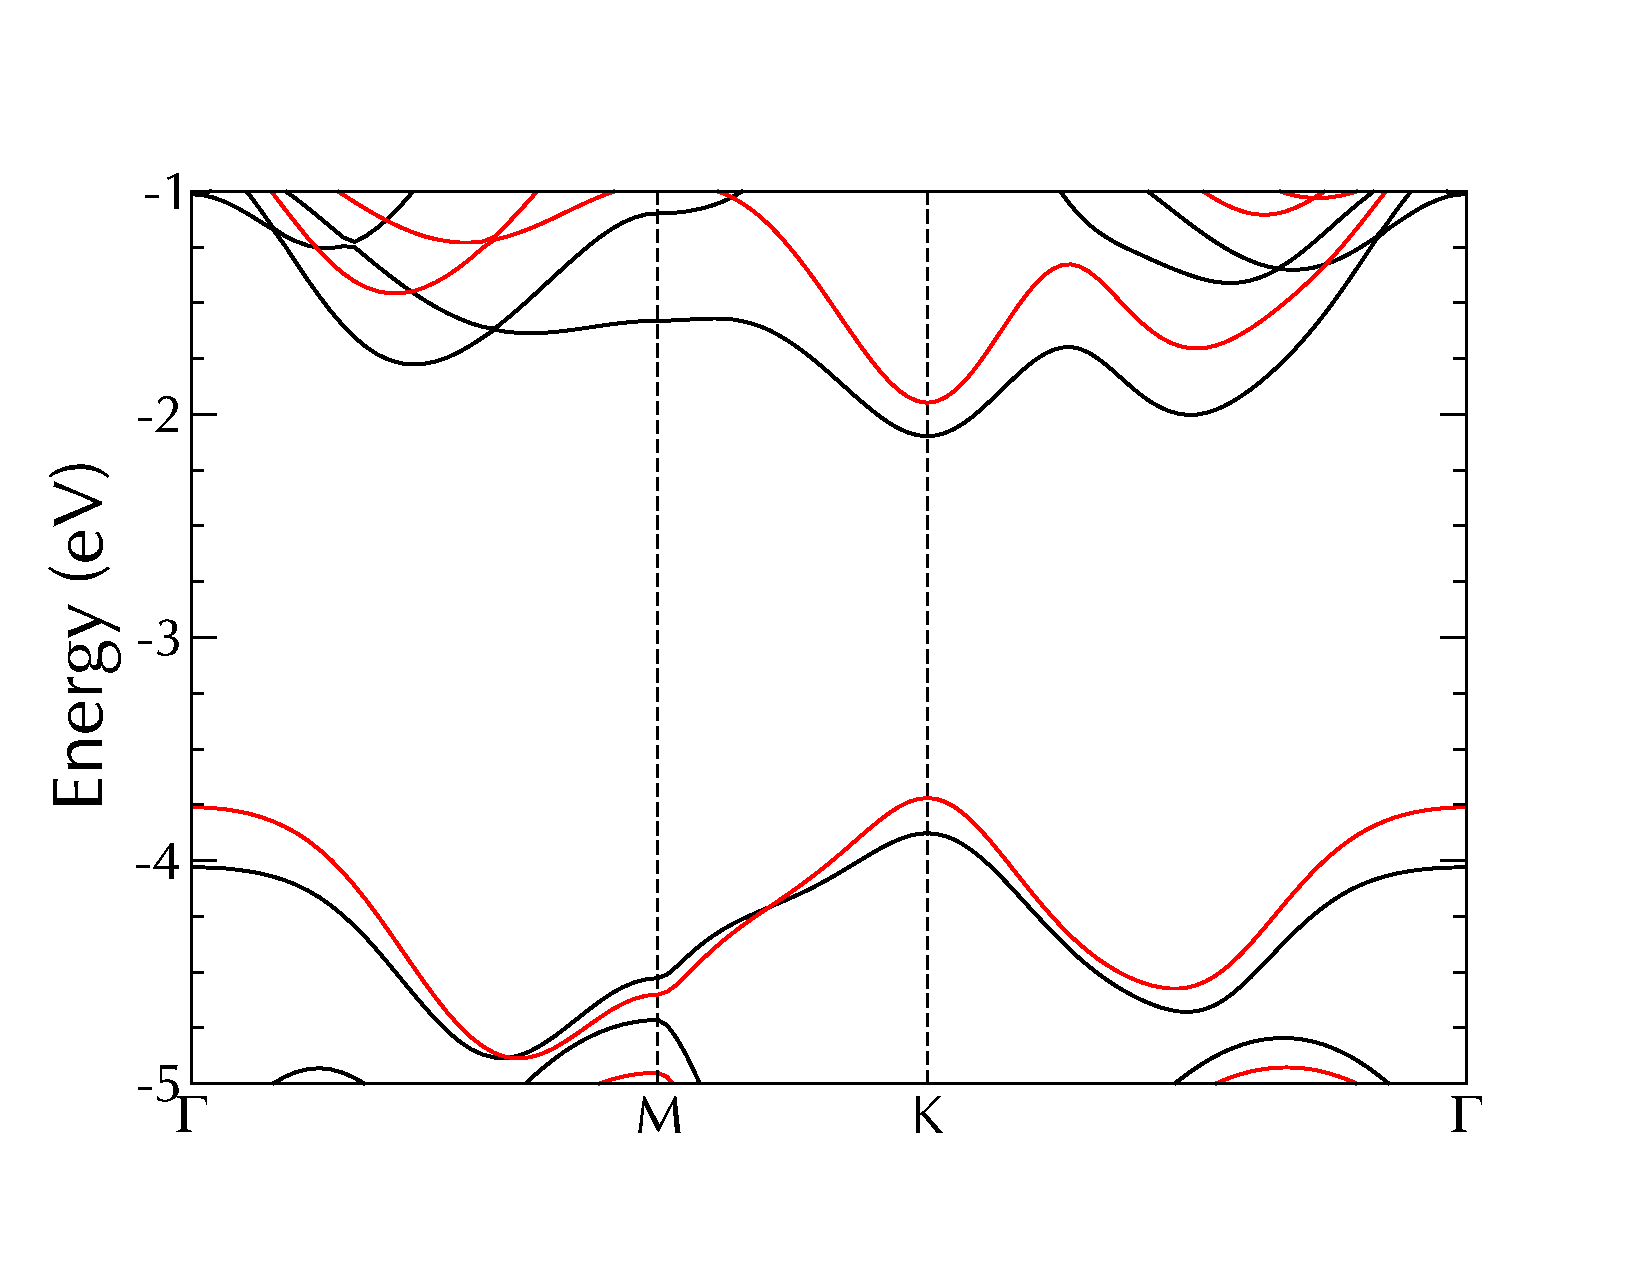
\includegraphics[width=\textwidth]{img/compare-mos2_ws2.pdf}
	\caption{Example of a monolayer MoS$_2$ band structure compared with a WS$_2$ band structure plotted using \texttt{vaspirin -compare -ref 0 0 -plot}. Black lines are from the first band structure (in this case, MoS$_2$) and red lines are from the second band structure (WS$_2$).}
	\label{fig:compare-bs}
\end{figure}

\marginlabel{Interpreting the figure:} Bands from the second OUTCAR are displayed in red, while bands from the first OUTCAR are displayed in black. \texttt{vaspirin} does not yet supports changing colors in bands. Pay attention to the reference: if nothing is specified within the \texttt{-ref} flag, the valence bands maxima from both OUTCARs will be set as the 0 eV reference.

\section{Other results}

\texttt{vaspirin} also allows users to plot using the \texttt{matplotlib} Python 3 library. Sample results for the usage of this method are shown below.

\subsection{Standard density of states with \texttt{-pyplot}}

\marginlabel{Density of states:}
\begin{figure}[h!]
\centering
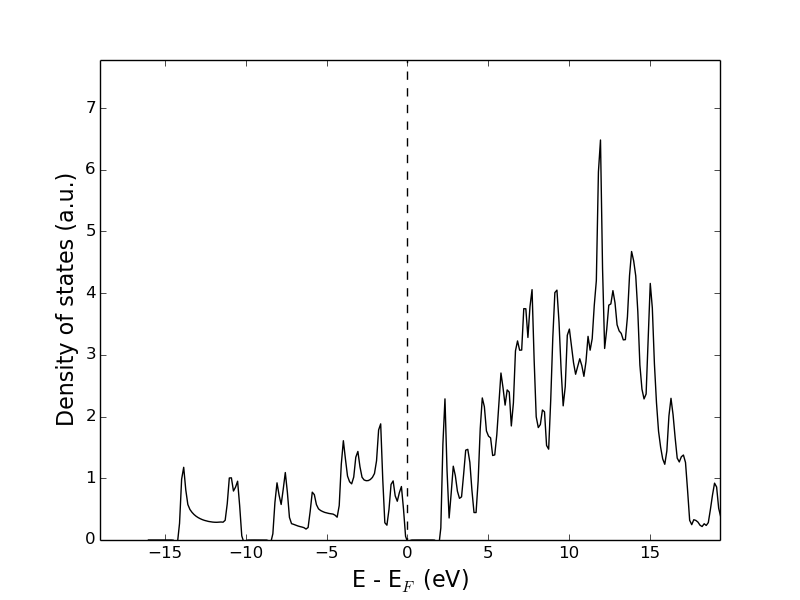
\includegraphics[width=0.90\columnwidth]{img/dos.png}
\caption{Example of result using -dos -pyplot tags.}
\label{fig:dos_pyplot}
\end{figure}


\subsection{Standard band structure with \texttt{-pyplot}}

\marginlabel{Band structure:}
\begin{figure}[h!]
\centering
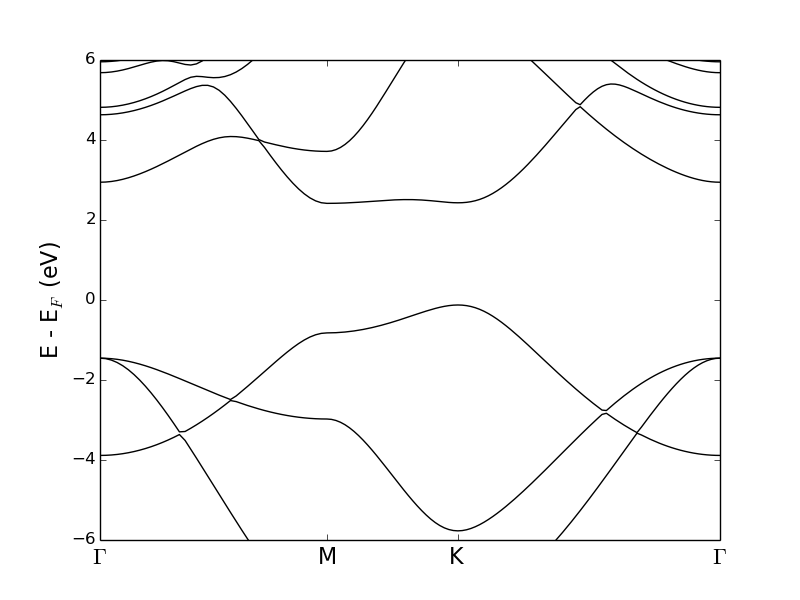
\includegraphics[width=.9\columnwidth]{img/BandStructure.png}
\caption{Example of result using -bs -pyplot tags.}
\label{fig:bs_pyplot}
\end{figure}

\subsection{BS + DOS plot with \texttt{-pyplot}}

\marginlabel{Band structure with DOS:}

\begin{figure}[h!]
\centering
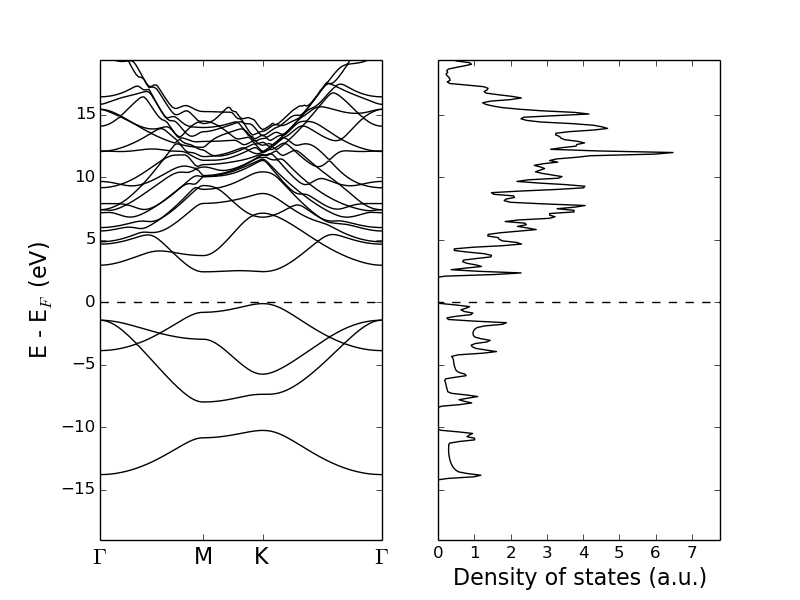
\includegraphics[width=.9\linewidth]{img/bsdos.png}
\caption{Example of result using -bs -dos -pyplot tags.}
\label{fig:bsdos_pyplot}
\end{figure}

\end{document}
